\documentclass[11pt, a4paper]{article}
\usepackage{pdfpages}
\usepackage{parallel}
\usepackage[T2A]{fontenc}
%\usepackage{ucs}
\usepackage[utf8]{inputenc}
\usepackage[english,russian]{babel}
\usepackage{hyperref}
\usepackage{rotating}
\usepackage[inner=2cm,top=1.8cm,outer=2cm,bottom=2.3cm,nohead]{geometry}
%\usepackage{listings}
\usepackage{graphicx}
\usepackage{wrapfig}
\usepackage{longtable}
\usepackage{indentfirst}
\usepackage{array}
\usepackage{tikzsymbols}
\usepackage{soul}
\usepackage[ruled,vlined]{algorithm2e}
\usepackage{qrcode}
\counterwithout{figure}{section} 

\usepackage{url}
\makeatletter
\g@addto@macro{\UrlBreaks}{\UrlOrds}
\makeatother

\newcolumntype{P}[1]{>{\raggedright\arraybackslash}p{#1}}
\frenchspacing
%\usepackage{fixltx2e} %text sub- and superscripts
\usepackage{icomma} % коскі ў матэматычным рэжыме
%\PreloadUnicodePage{4}

\newcommand{\longpage}{\enlargethispage{\baselineskip}}
\newcommand{\shortpage}{\enlargethispage{-\baselineskip}}

\def\switchlang#1{\expandafter\csname switchlang#1\endcsname}
\def\switchlangbe{
\let\saverefname=\refname%
\def\refname{Літаратура}%
\def\figurename{Іл.}%
}
\def\switchlangru{
\let\saverefname=\refname%
\let\savefigurename=\figurename%
\def\refname{Литература}%
\def\figurename{Рис.}%
}
\def\switchlangen{
\let\saverefname=\refname%
\def\refname{References}%
\def\figurename{Fig.}%
}

\hyphenation{admi-ni-stra-tive}
\hyphenation{ex-pe-ri-ence}
\hyphenation{fle-xi-bi-li-ty}
\hyphenation{Py-thon}
\hyphenation{ma-the-ma-ti-cal}
\hyphenation{re-ported}
\hyphenation{imp-le-menta-tions}
\hyphenation{pro-vides}
\hyphenation{en-gi-neering}
\hyphenation{com-pa-ti-bi-li-ty}
\hyphenation{im-pos-sible}
\hyphenation{desk-top}
\hyphenation{elec-tro-nic}
\hyphenation{com-pa-ny}
\hyphenation{de-ve-lop-ment}
\hyphenation{de-ve-loping}
\hyphenation{de-ve-lop}
\hyphenation{da-ta-ba-se}
\hyphenation{plat-forms}
\hyphenation{or-ga-ni-za-tion}
\hyphenation{pro-gramming}
\hyphenation{in-stru-ments}
\hyphenation{Li-nux}
\hyphenation{sour-ce}
\hyphenation{en-vi-ron-ment}
\hyphenation{Te-le-pathy}
\hyphenation{Li-nux-ov-ka}
\hyphenation{Open-BSD}
\hyphenation{Free-BSD}
\hyphenation{men-ti-on-ed}
\hyphenation{app-li-ca-tion}

\def\progref!#1!{\texttt{#1}}
\renewcommand{\arraystretch}{2} %Іначай формулы ў матрыцы зліпаюцца з лініямі
\usepackage{array}

\def\interview #1 (#2), #3, #4, #5\par{

\section[#1, #3, #4]{#1 -- #3, #4}
\def\qname{LVEE}
\def\aname{#1}
\def\q ##1\par{{\noindent \bf \qname: ##1 }\par}
\def\a{{\noindent \bf \aname: } \def\qname{L}\def\aname{#2}}
}

\def\interview* #1 (#2), #3, #4, #5\par{

\section*{#1\\{\small\rm #3, #4. #5}}
\ifx\ParallelWhichBox\undefined%
    \addcontentsline{toc}{section}{#1, #3, #4}%
\else%
\ifnum\ParallelWhichBox=0%
    \addcontentsline{toc}{section}{#1, #3, #4}%
\fi\fi%

\def\qname{LVEE}
\def\aname{#1}
\def\q ##1\par{{\noindent \bf \qname: ##1 }\par}
\def\a{{\noindent \bf \aname: } \def\qname{L}\def\aname{#2}}
}

\newcommand{\interviewfooter}[1]{
\vskip 1em
\noindent \textit{#1}
}

\AtEndDocument{\vfill\centering \qrcode{https://github.com/fiowro/mouses/blob/main/\jobname.pdf}}

\switchlang{en}
\begin{document}

\title{1981 -- Xerox Alto Optical Mouse}
\date{}
\maketitle
\selectlanguage{english}
In September 1986, Xerox Corporation announced the EWS 4800 UNIX workstation. This computer was designed as a workstation for engineers to improve the efficiency of solving problems such as software development, computer-aided design, scientific and engineering calculations, and the collection and analysis of experimental data \cite{yt}. The computer was equipped with a graphical multi-window interface and a large 20-inch $1280 \times 1024 \times 256$ display. This powerful workstation came with the Xerox Alto Mouse (figure \ref{fig:XeroxAltoPic}).

The specially produced chip and other parts were incorporated into the standard Xerox Alto mouse housing \cite{vlsi82}.

\begin{figure}[h]
    \centering
    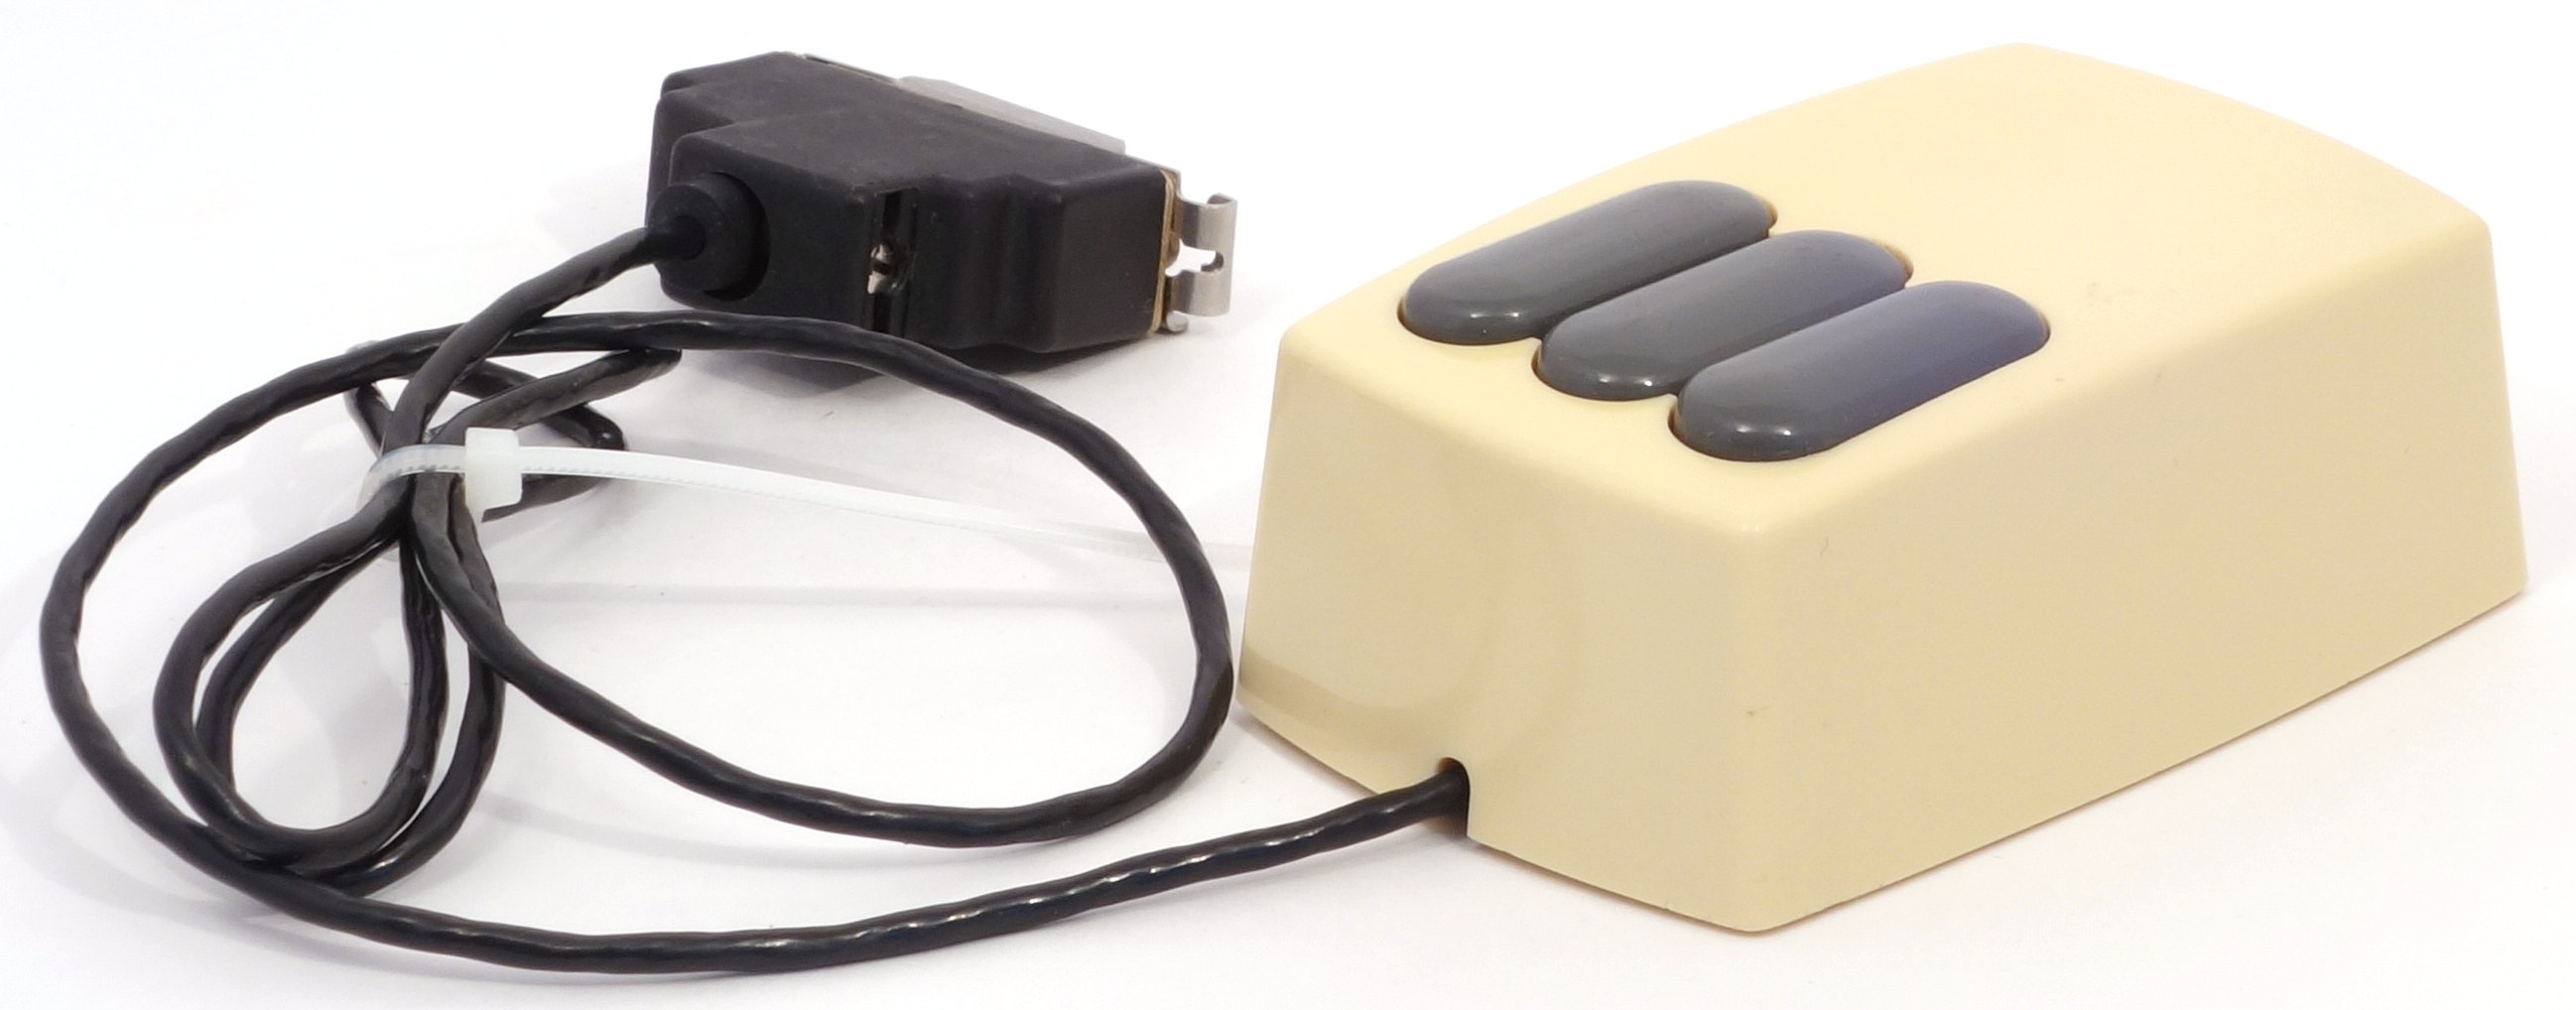
\includegraphics[scale=0.7]{1981_xerox_alto_mouse/pic_30.jpg}
    \caption{Xerox Alto Optical Mouse}
    \label{fig:XeroxAltoPic}
\end{figure}

The mousepad was paper, sold in packs of 25 sheets \cite{pad}. The pattern was a
hexagonal array of light dots in a dark field, and was absolutely usable being duplicated by a copier. The reconstructed pad can be seen on fig. \ref{fig:XeroxAltoPad}.

\begin{figure}[h]
    \centering
    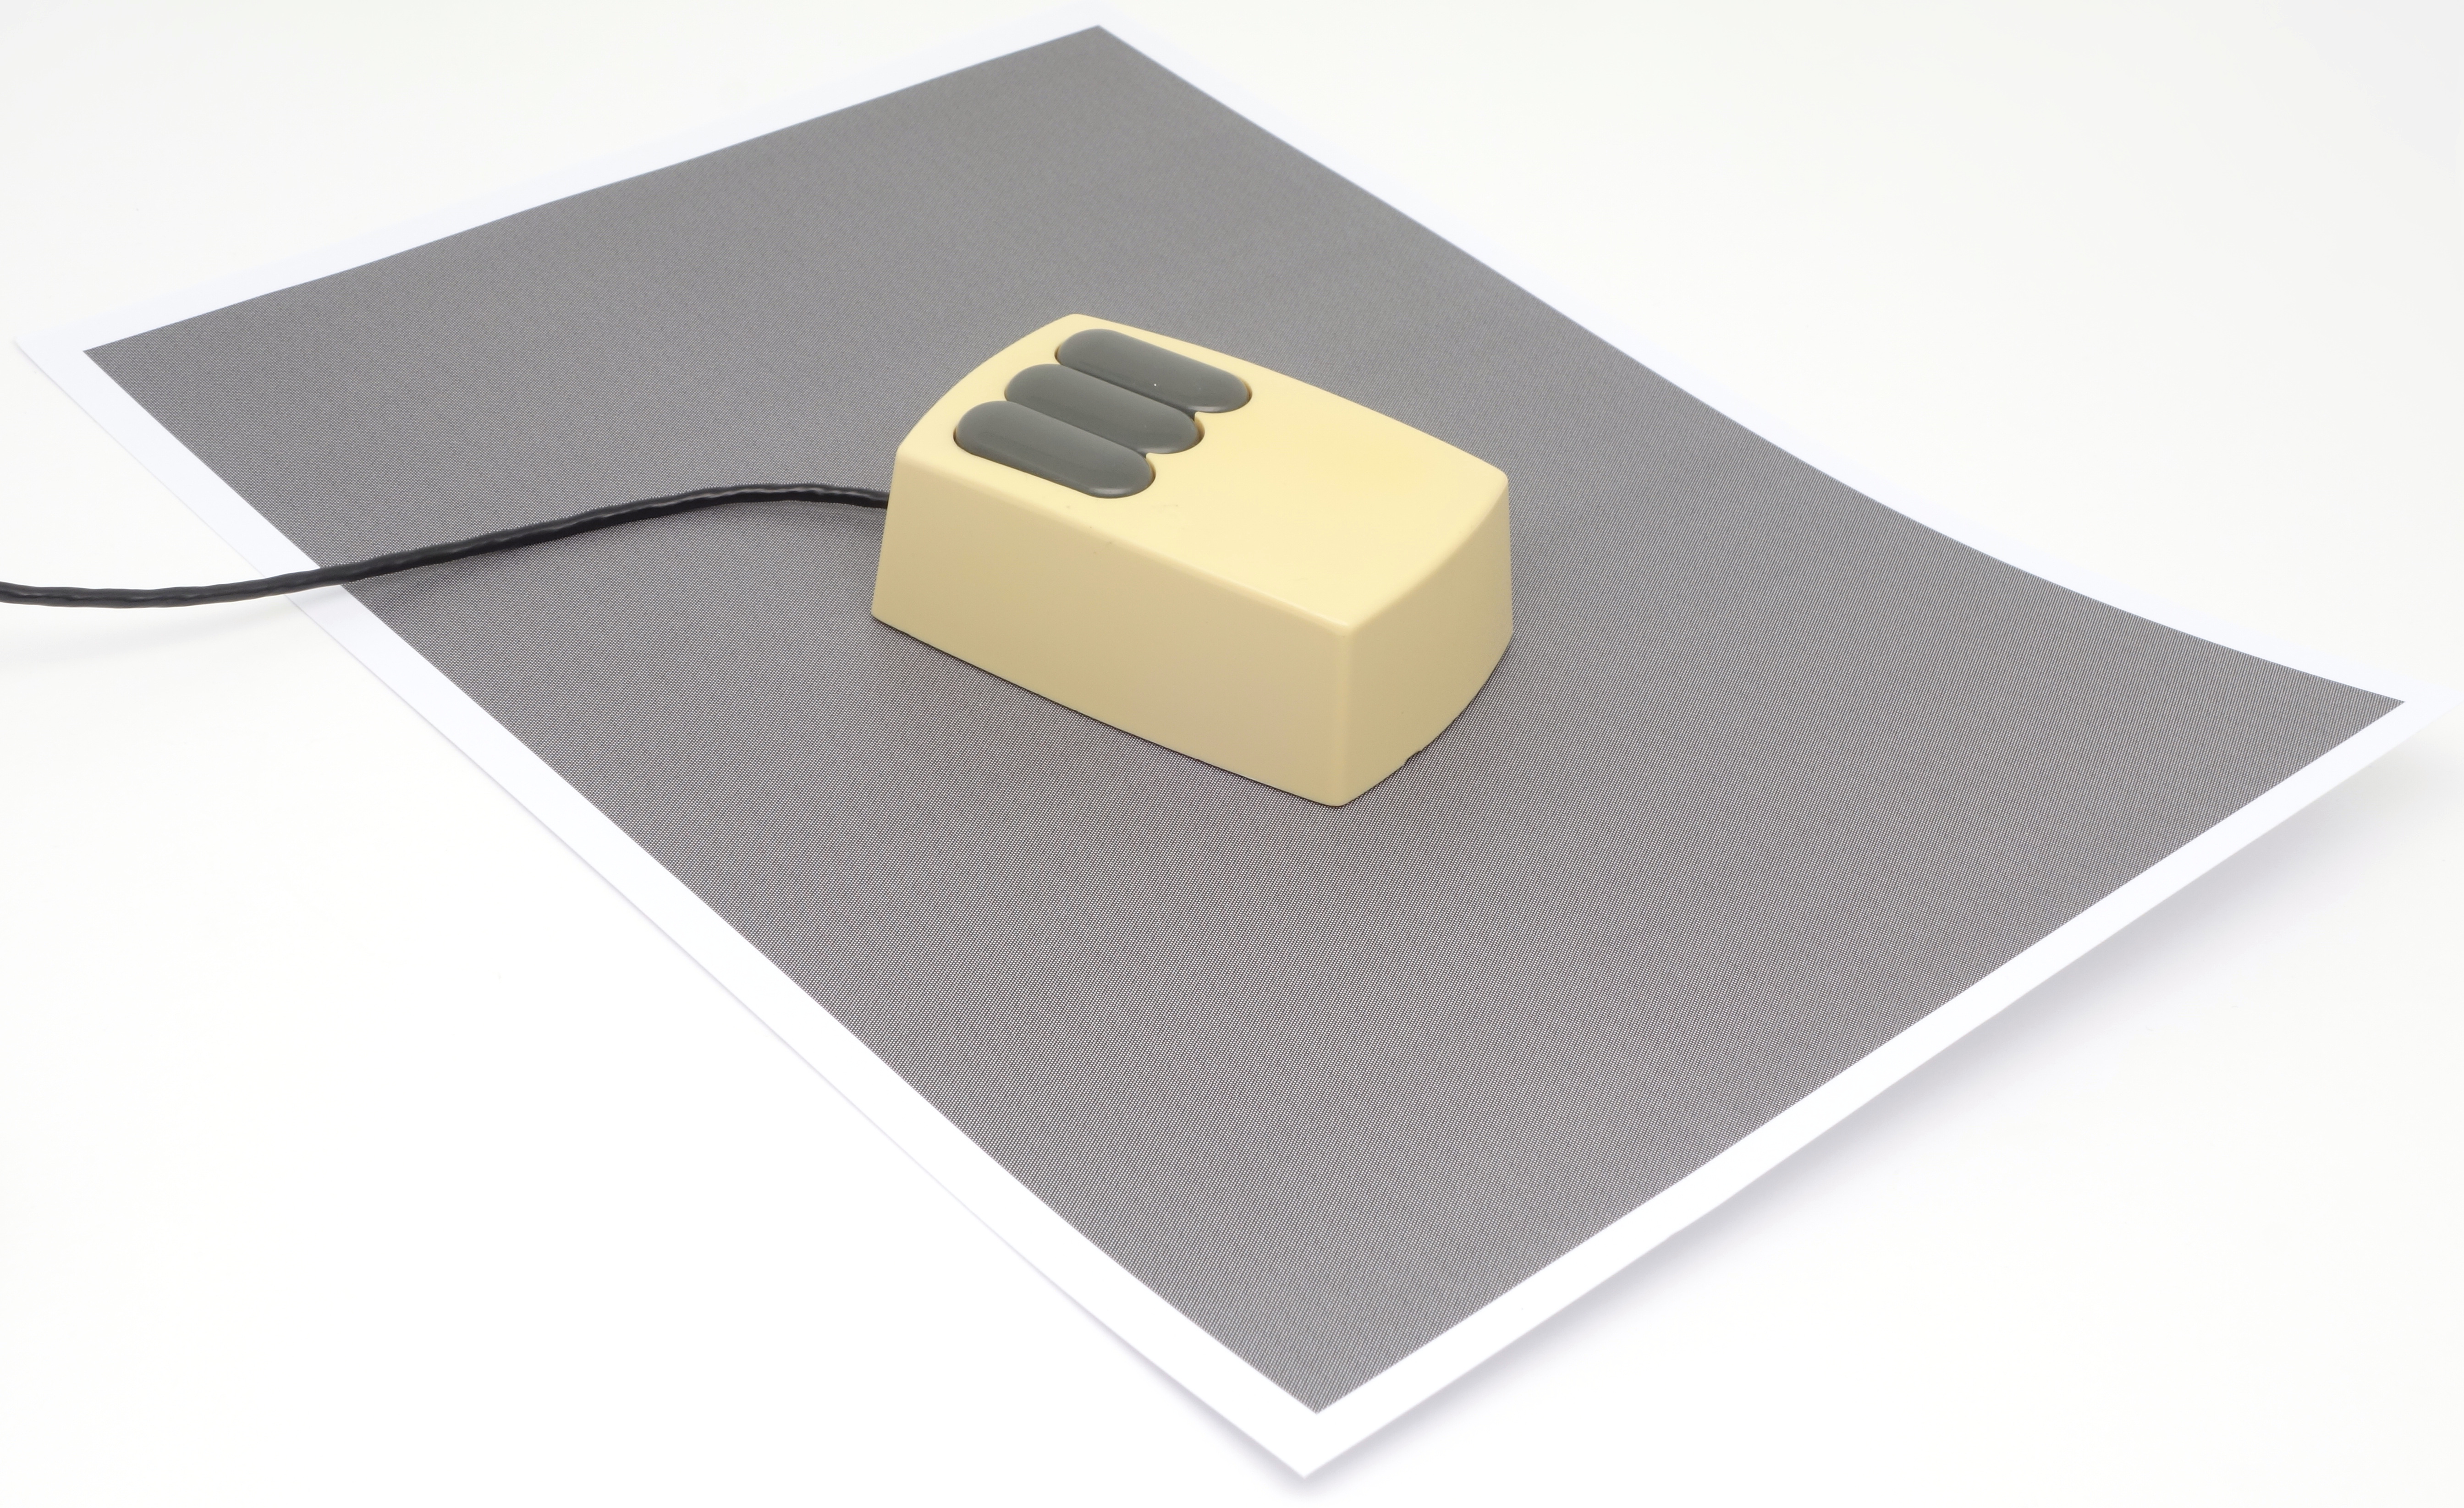
\includegraphics[scale=0.4]{1981_xerox_alto_mouse/pad_30.jpg}
    \caption{Xerox Alto Optical Mouse on a reconstructed pad}
    \label{fig:XeroxAltoPad}
\end{figure}

The name of the mouse “Alto Mouse” is highlighted on the upper side of the case with two triangular stylized mice in outlines and solid lines. The bottom side shows that this is an optical mouse (figure \ref{NecAltoTopAndBottom}), which largely repeats the external design solutions of the Mouse Systems mice of the same period and is intended for use with a special mirror pad \cite{photo}.

\begin{figure}[h]
    \centering
    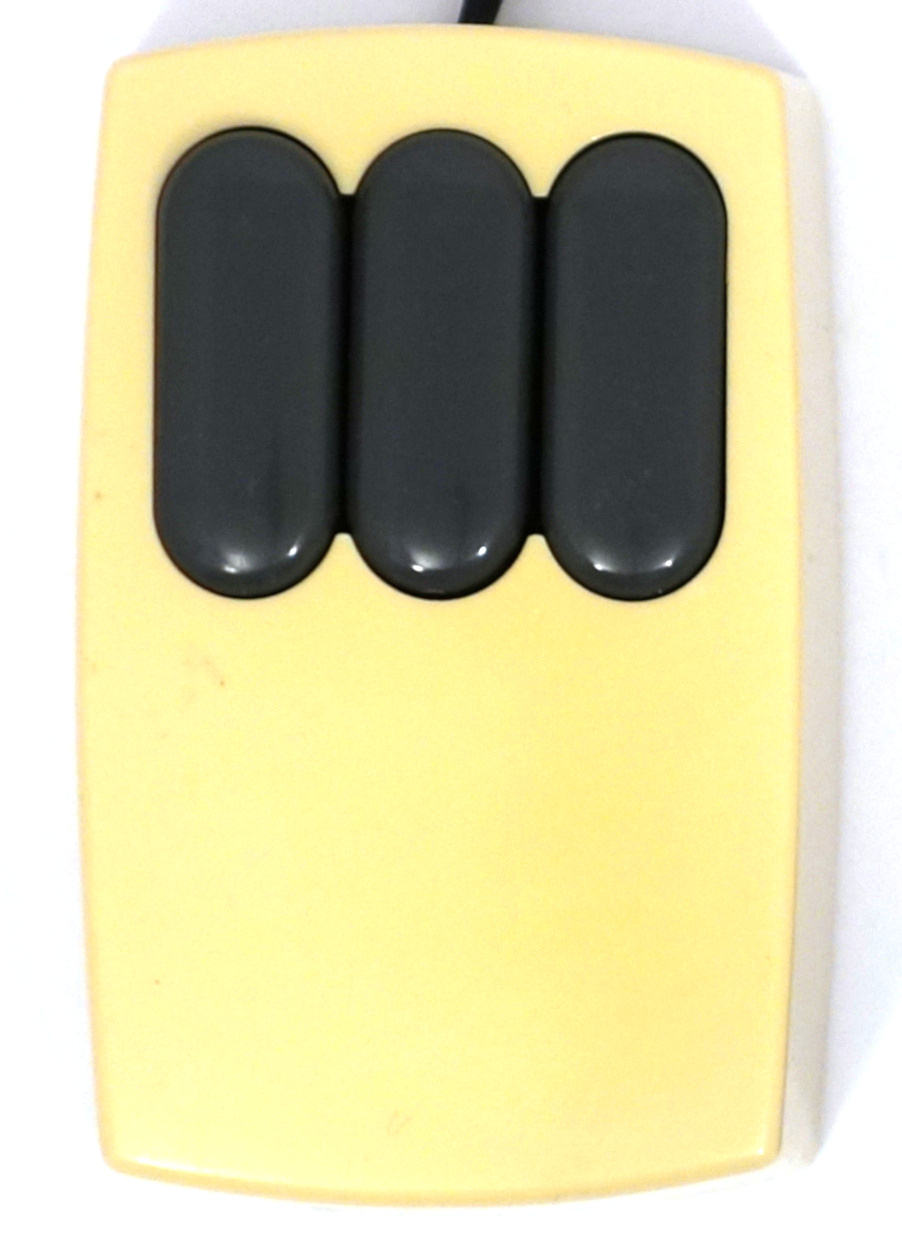
\includegraphics[scale=0.5]{1981_xerox_alto_mouse/top_30.jpg}
    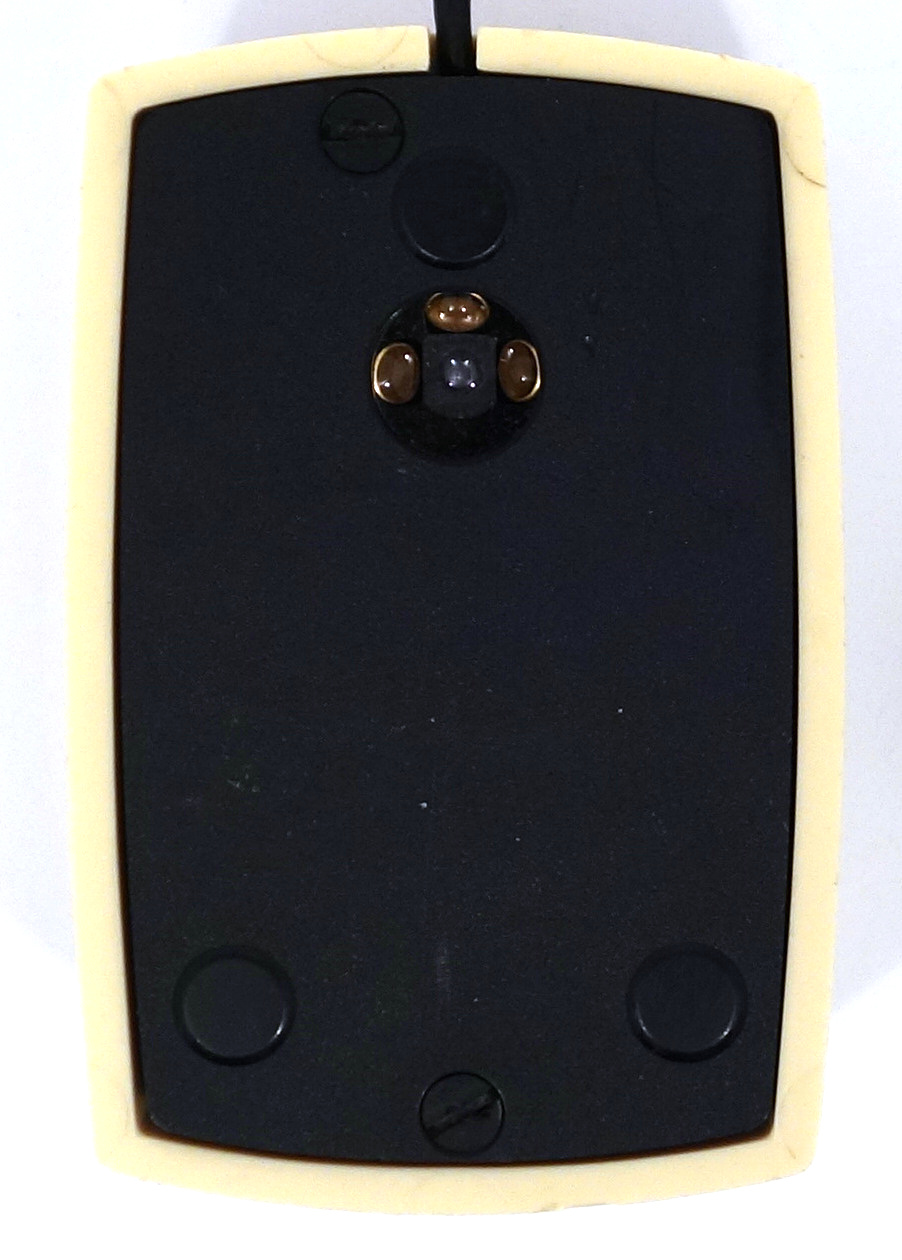
\includegraphics[scale=0.5]{1981_xerox_alto_mouse/bottom_30.jpg}
    \caption{Xerox Alto Optical Mouse, top and bottom views}
    \label{NecAltoTopAndBottom}
\end{figure}

In terms of size, the manipulator is an optical cursor control device typical for the 80s (figure \ref{fig:NecAltoSize}).

\begin{figure}[h]
    \centering
    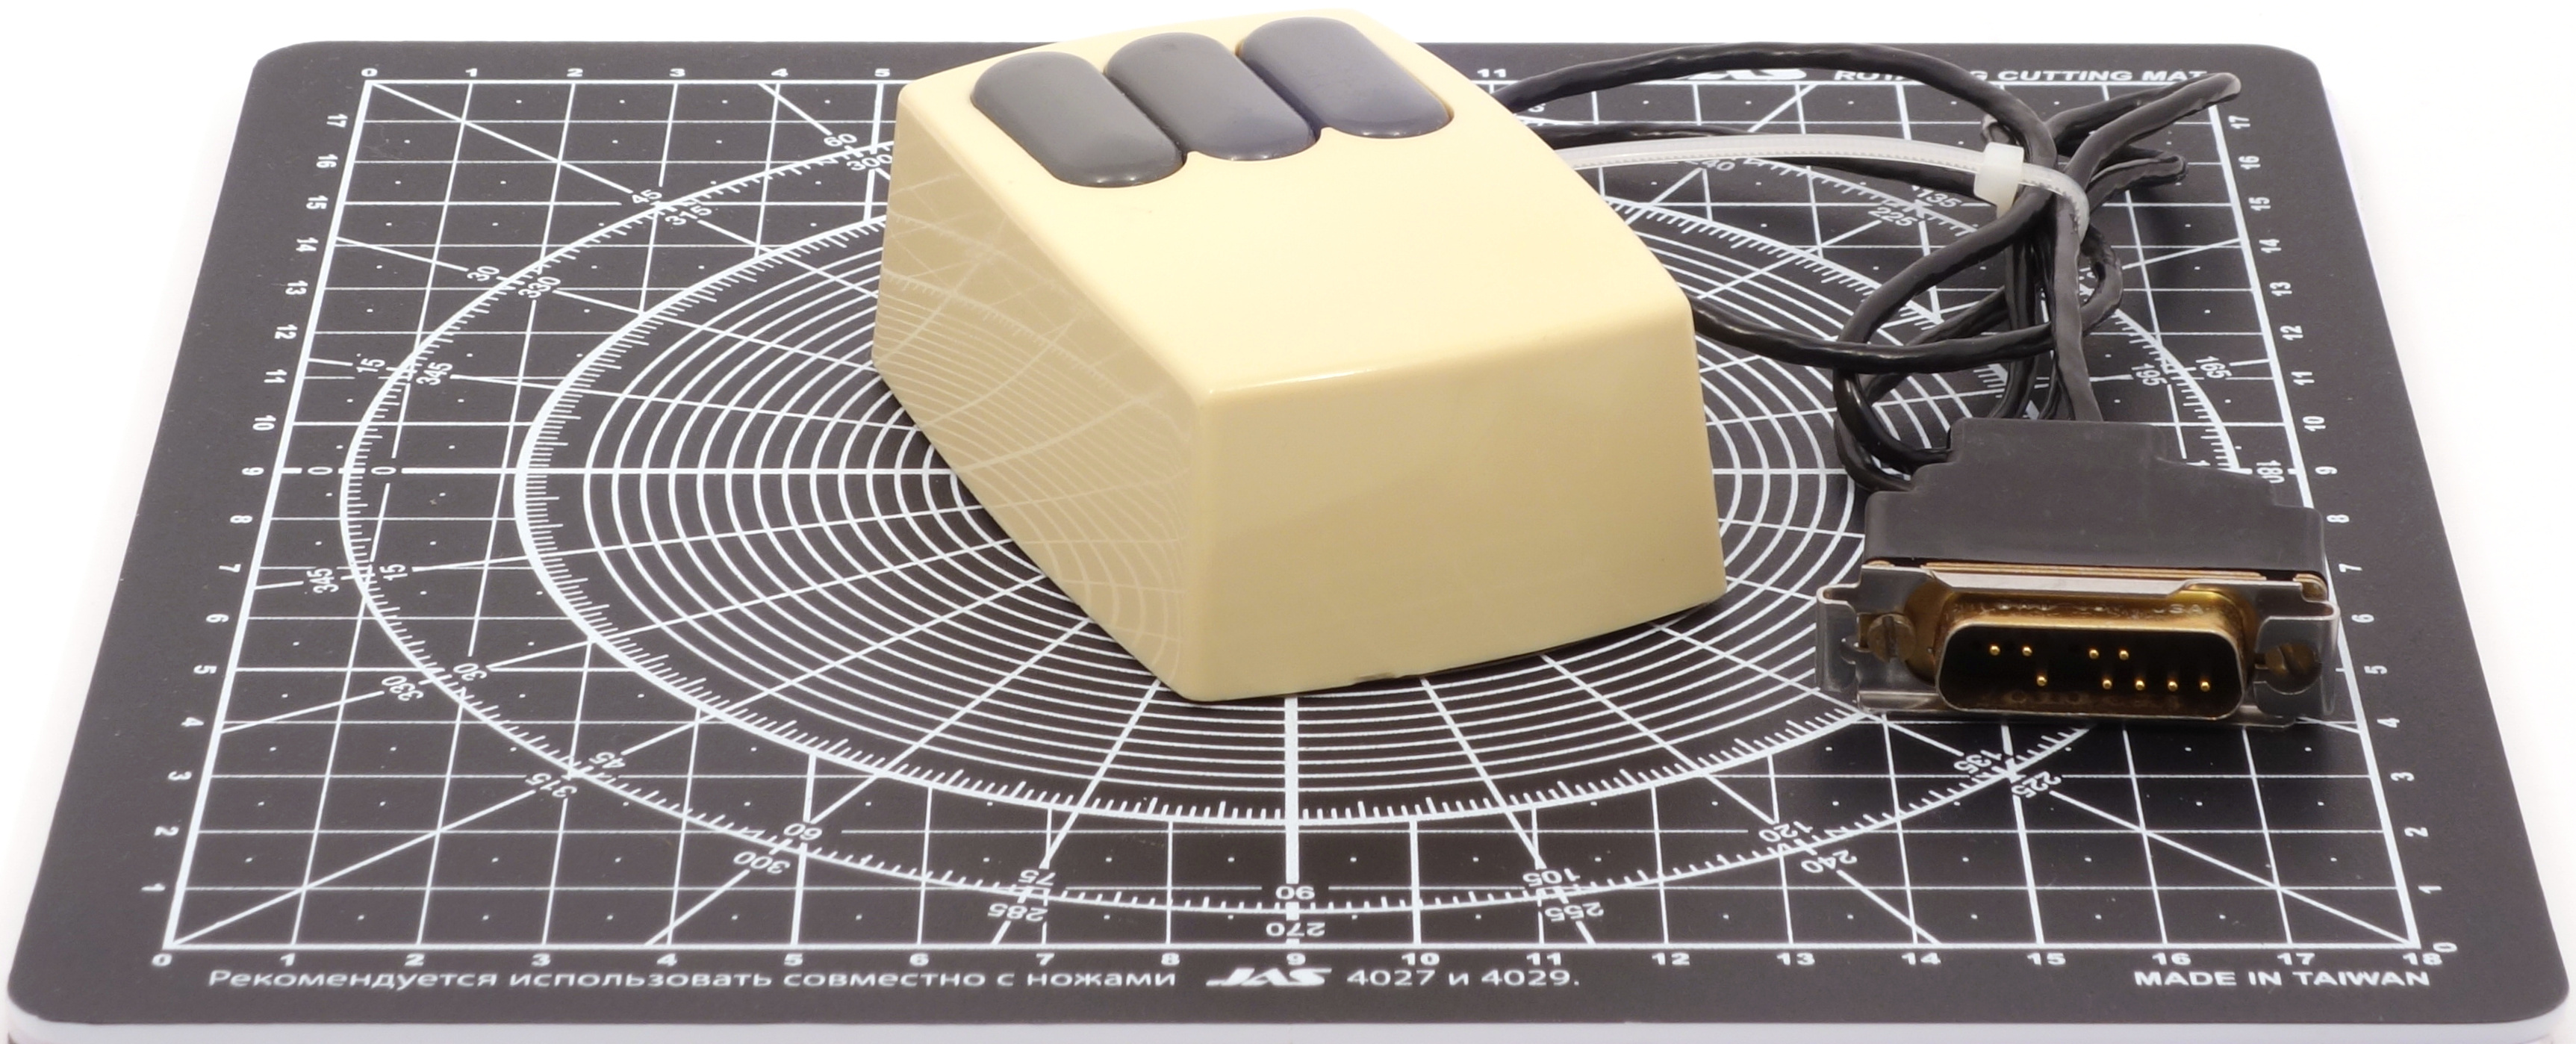
\includegraphics[scale=0.4]{1981_xerox_alto_mouse/size_15.jpg}
    \caption{Xerox Alto Optical Mouse on a graduated pad with a grid step of 1~cm}
    \label{fig:NecAltoSize}
\end{figure}

In terms of ergonomics, the exterior of the Alto Mouse has a strong industrial design. At the same time, a large number of corners and flat edges are partly compensated by rounded joints of the edges in the part of the body closest to the user and convex long buttons conveniently located within the reach of the fingers (figure \ref{fig:NecAltoHand}).

\begin{figure}[h]
    \centering
    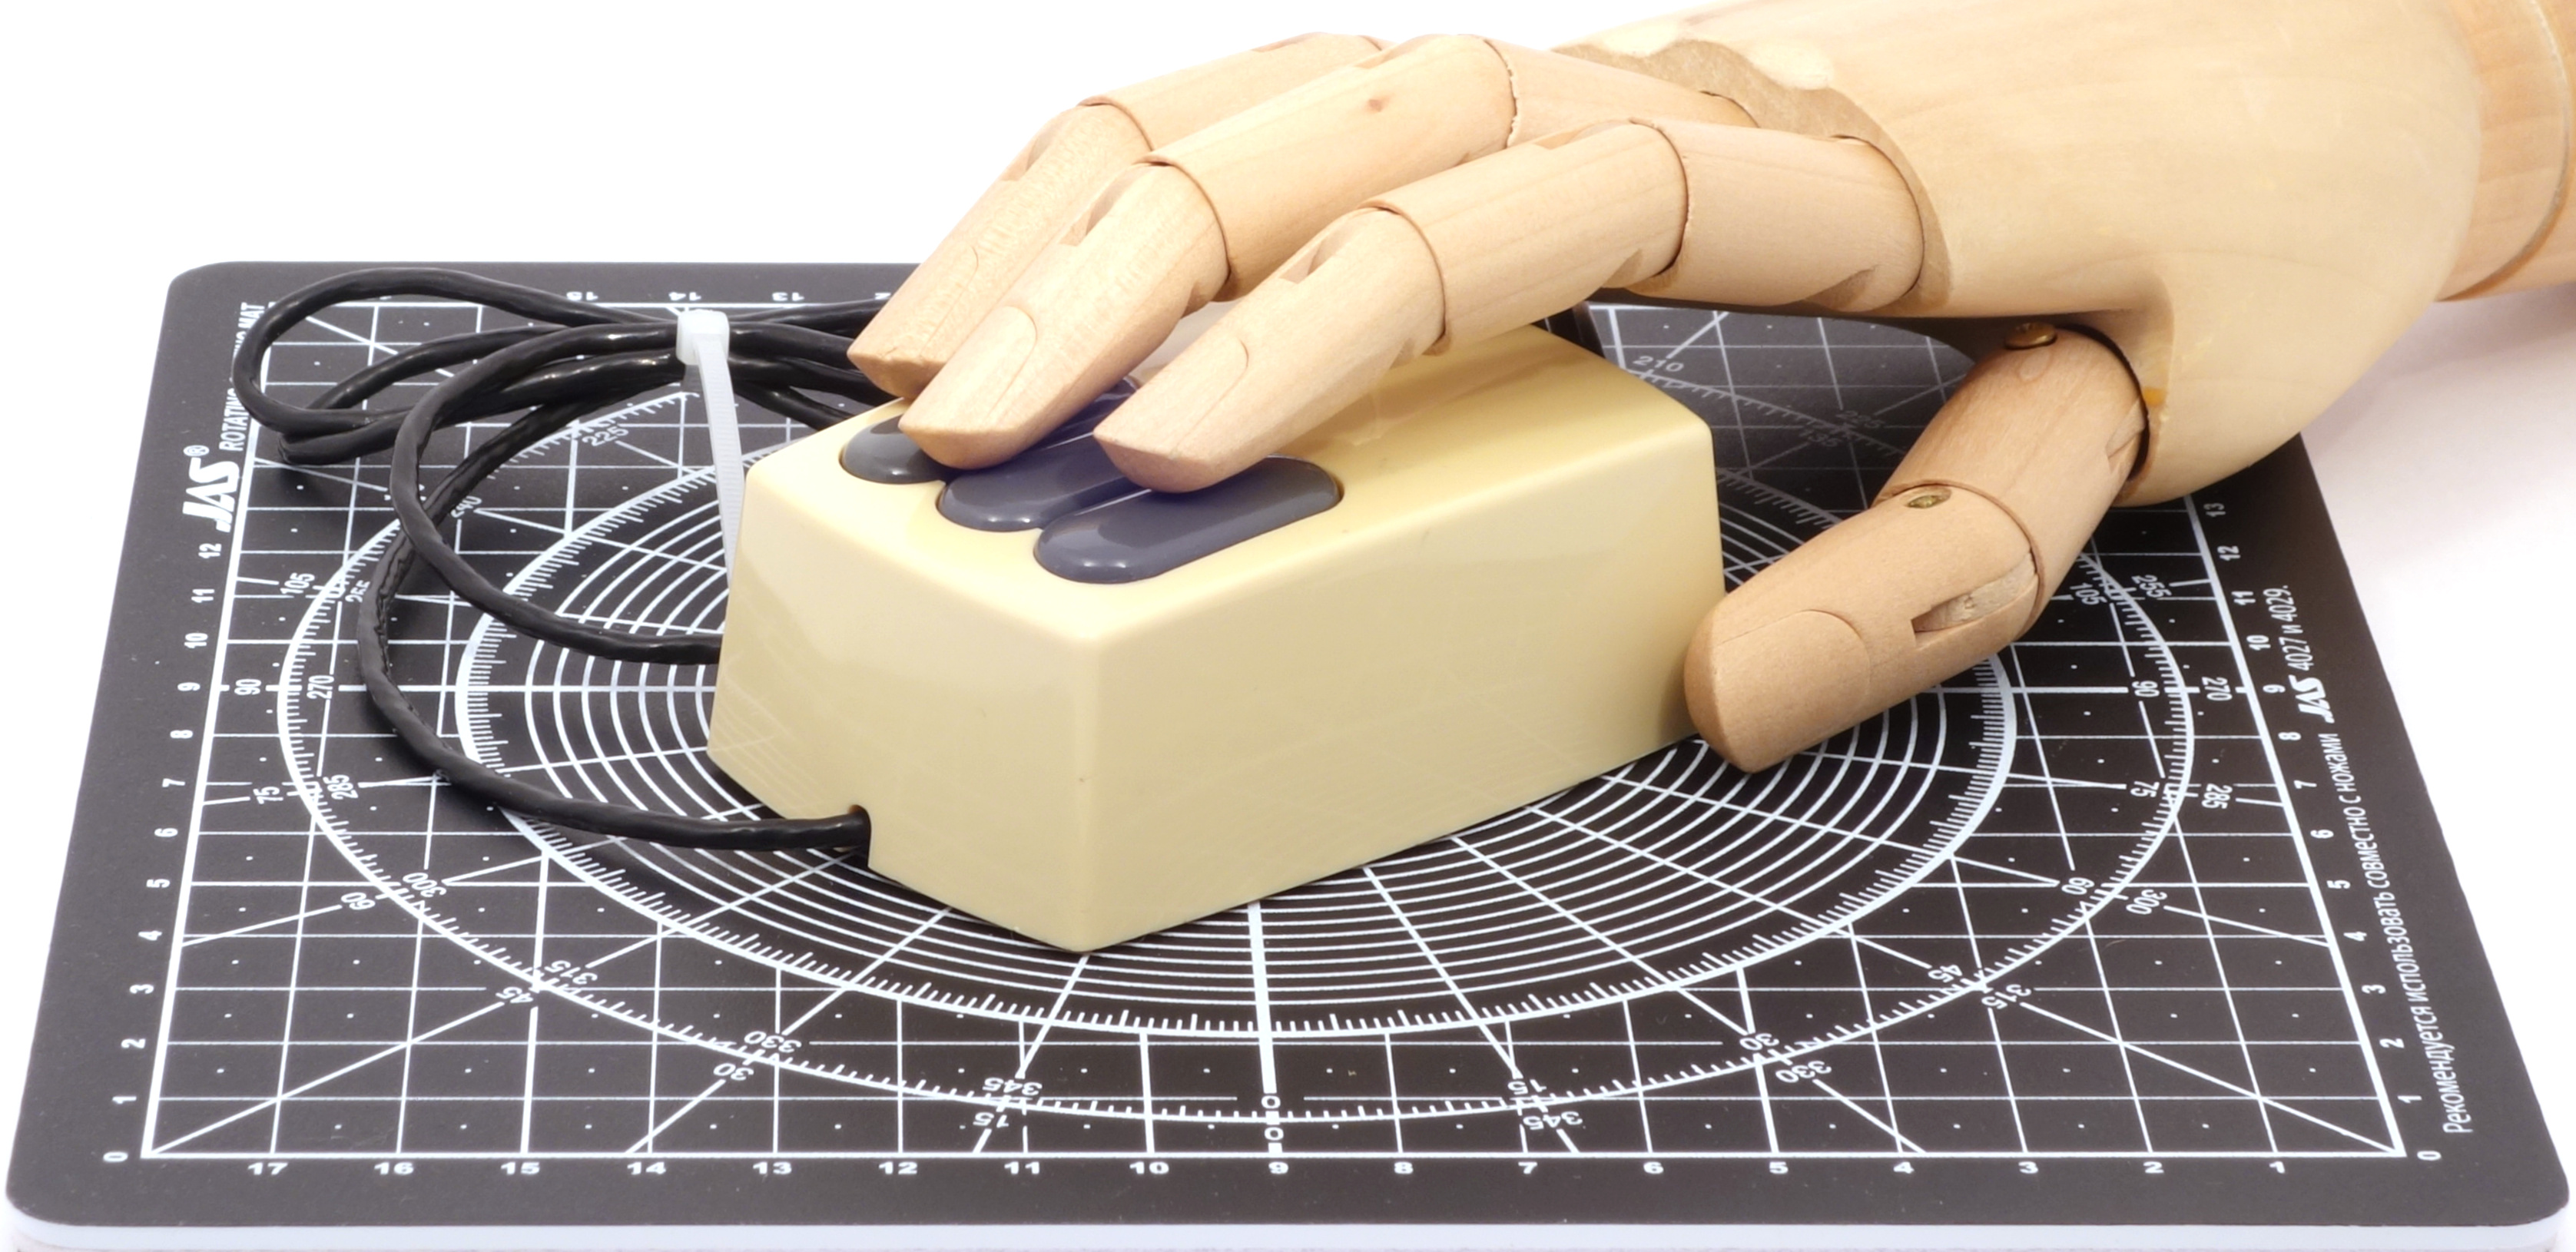
\includegraphics[scale=0.4]{1981_xerox_alto_mouse/hand_30.jpg}
    \caption{Xerox Alto Optical Mouse with a human hand model}
    \label{fig:NecAltoHand}
\end{figure}

Xerox Alto Mouse has a DIN connector and belongs to the Bus Mouse category according to the connection interface. A feature of such mice is that the optocoupler signals are processed not by a chip in the mouse case, but by a special adapter in the computer system unit; therefore, this mouse is powered by the computer without a separate power supply, unlike many early optical models that were connected to the serial port of the IBM PC.

\begin{figure}[h]
    \centering
    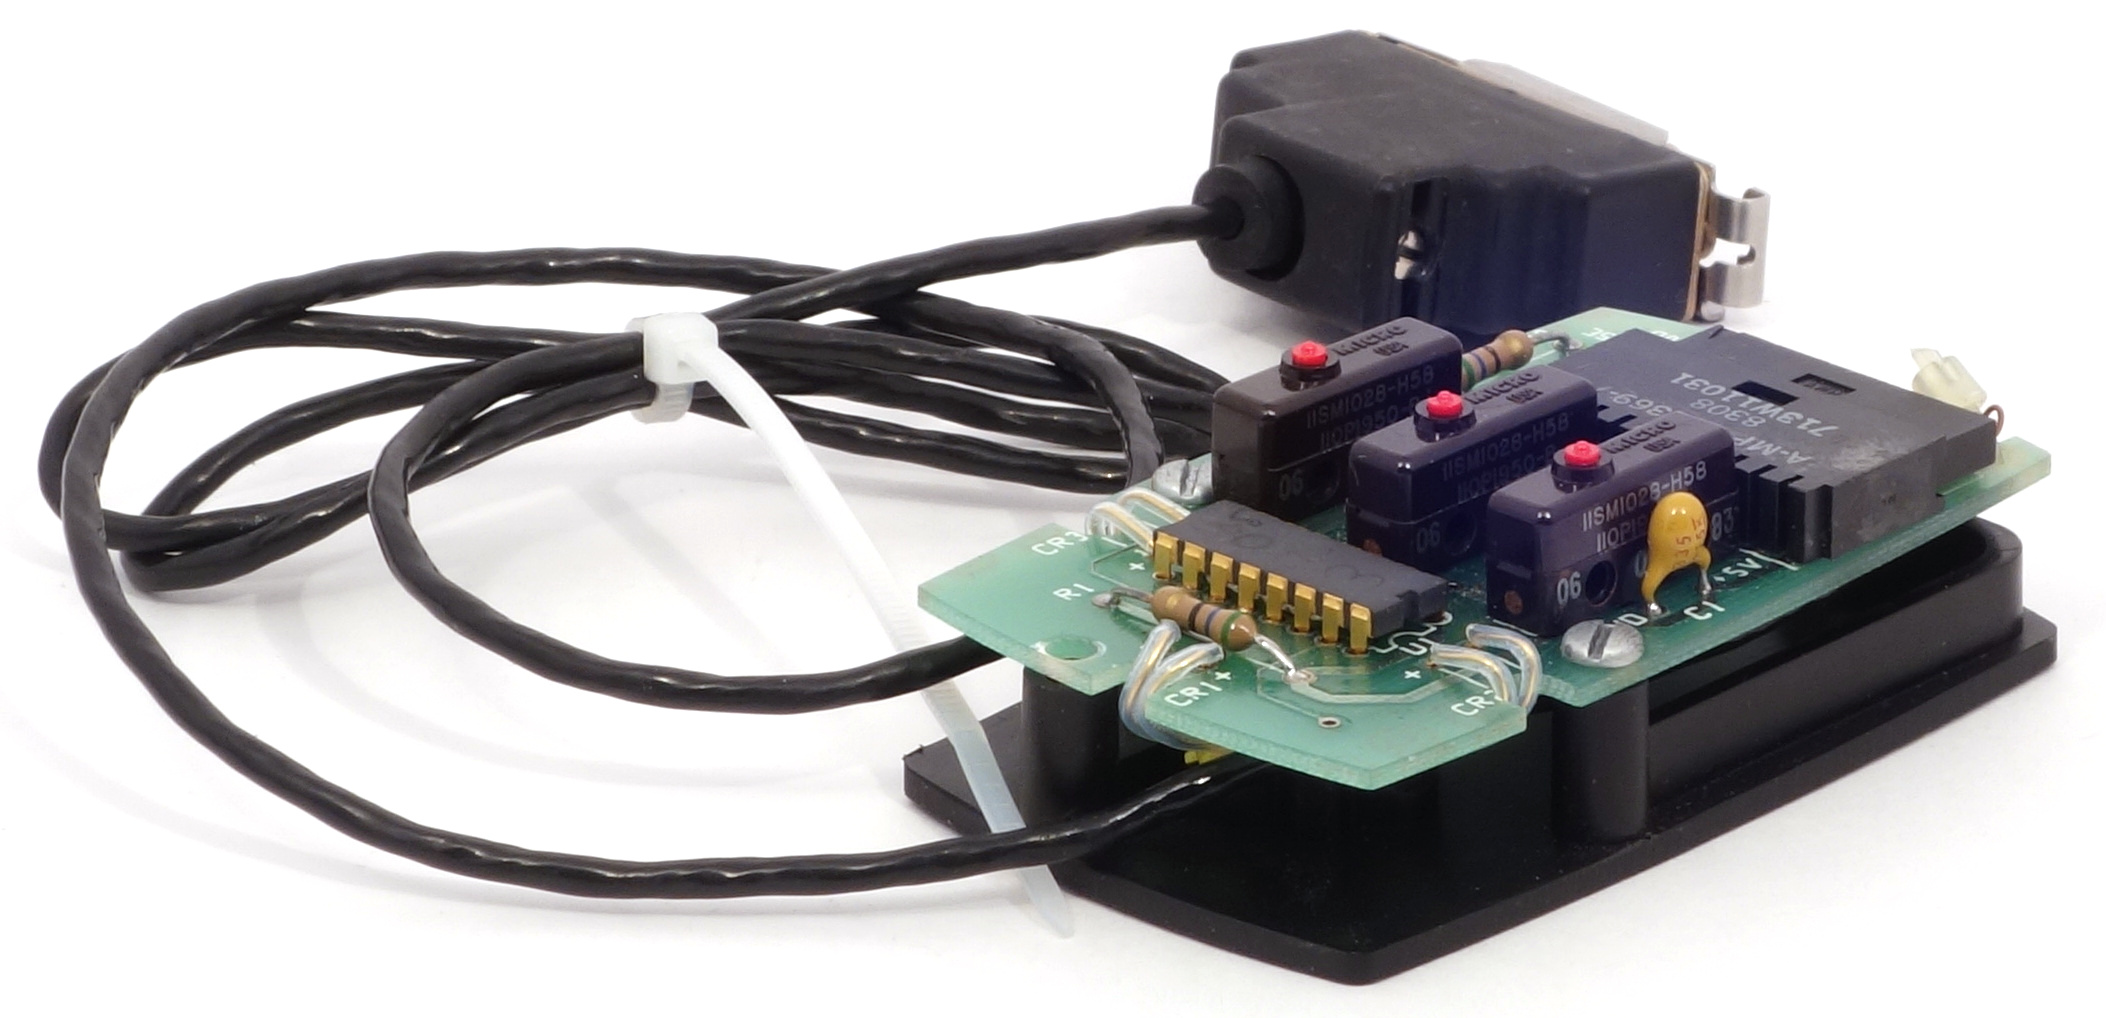
\includegraphics[scale=0.8]{1981_xerox_alto_mouse/inside_60.jpg}
    \caption{Xerox Alto Optical Mouse disassembled}
    \label{fig:NecAltoInside}
\end{figure}

Mouse internals are shown on figure \ref{fig:NecAltoInside}. You can see the original design of this optical mouse. Unlike most optical mice of the 80s, it is not a direct copy of the Mouse Systems device, which has become a prototype for subsequent manipulators of this type.

\begin{thebibliography}{9}
\bibitem {vlsi81} R.\,F. Lyon. The Optical Mouse, and an Architectural Methodology for
Smart Digital Sensors // VLSI DESIGN, August 1981. - p. 20--30. \url{https://www.dicklyon.com/tech/OMouse/OpticalMouse-Lyon.pdf}
\bibitem {vlsi82} R.\,F. Lyon, M.\,P. Haeberli. Designing and Testing The Optical Mouse // VLSI DESIGN, January/February, 1982. - p. 20--30. \url{https://www.dicklyon.com/tech/OMouse/DesigningTestingOMouse.pdf}
\bibitem{pad} R.\,F. Lyon The Optical Mouse: Early Biomimetic Embedded Vision / Advances in Embedded Computer Vision, Nov 2014, pp.3-22 \url{https://static.googleusercontent.com/media/research.google.com/ru//pubs/archive/43260.pdf}
\bibitem{mouses} Xerox Mice. oldmouse.com \url{https://web.archive.org/web/20210418000634/http://oldmouse.com/mouse/xerox/alto.shtml}
\end{thebibliography}
\end{document}
